\chapter{Асимптотическое поведение орбит динамических систем. Существование орбит более высокого периода.}
\section{Предсказание судьбы орбиты для данного отображения}
Иногда исследование эволюции всех орбит --- легкая задача. Простейшим примером является модель неограниченного роста популяции,
которая суть геометрическая прогрессия. 
\exmpl{}{
    Рассмотрим отображение \(\overline{x} = x^2\), легко предсказать судьбу траектории всех точек на оси \(x\).
    Найдем неподвижные точки отображения{:}
    \[
        x = x^2 \implies x = 0,\, x = 1
        \]
    \begin{itemize}
        \item орбита \(x = 0{:} \ \ 0,\, 0,\, 0, \dots \) 
        \item орбита \(x = 1{:} \ \ 1,\, 1,\, 1, \dots \)
        \item орбита \(x = -1{:} \ \ -1,\, 1,\, 1,\, \dots\) --- преднеподвижная точка
    \end{itemize}
    Рассмотрим судьбу орбит отображения \(\overline{x} = x^2 \) для \( \vert x \vert < 1,\, x \not = 0{:}\)
    \[
        x,\, x^2,\, x^4,\, x^8,\, \dots ,\, x^{2^n}, \dots \]
    \[
        x_0 = \frac{1}{2},\, x_1 = \frac{1}{4},\, x_2 = \frac{1}{16},\, \dots ,\, x_{n} = \frac{1}{2^{2^n}}\]
    Рассмотрим судьбу орбит отображения \(\overline{x} = x^2 \) для \( \vert x \vert > 1{:}\)
    \[
        x,\, x^2,\, x^4,\, x^8,\, \dots ,\, x^{2^n}, \dots \ \ x_{n} \to \infty\]
}{}

\exmpl{}{
    Рассмотрим динамическую систему \(\overline{x} = x^2 - 1{:}\)
    \begin{itemize}
        \item \(x = x^2 - 1 \implies x_{1, 2} = \frac{1 \pm \sqrt{5} }{2} - \text{две неподвижные точки}\)
        \item имеется периодическая орбита \(x = 0\) периода 2. 
        \item предпериодическая точка \(\sqrt{2} \), ее орбита: \(\sqrt{2},\, 1,\, 0,\, -1,\, 0,\, \dots   \) 
    \end{itemize}
    \exsz{}{
        Найти еще несколько предпериодических орбит.
    }{}
}{}
\subsection{Диаграмма Ламерея}
Удобным способом исследования орбит динамических систем является \textit{диаграмма Ламерея} (итерационная диаграмма)
\\[2mm]
\textbf{Алгоритм{:} }
\begin{itemize}
    \item строится график отображения (дискретной динамической системы) и биссектриса в 1 и 3 четвертях
    \item перемещаемся по некоторой "лестнице" \, (подробно в следующей лекции)
\end{itemize}
Рассмотрим отображение \(\overline{x} = x^2 - 1 \) и орбиту точки \(x_0 = 0.5{:}\)
\begin{itemize}
    \item[] \(x_0 = 0.5000\)
    \item[] \(x_1 = 0.5^2 - 1 = -0.7500\)
    \item[] \(x_2 = -0.4375\)
    \item[] \(x_3 = -0.8086\)
    \item[] \(\vdots\)
    \item[] \(x_{20} = 0.0000 \)
    \item[] \(x_{21} = -1.0000 \)
    \item[] \(x_{22} = 0.0000 \)
\end{itemize}
- - - - тут будут рисунки - - - -


\begin{figure}[h]
    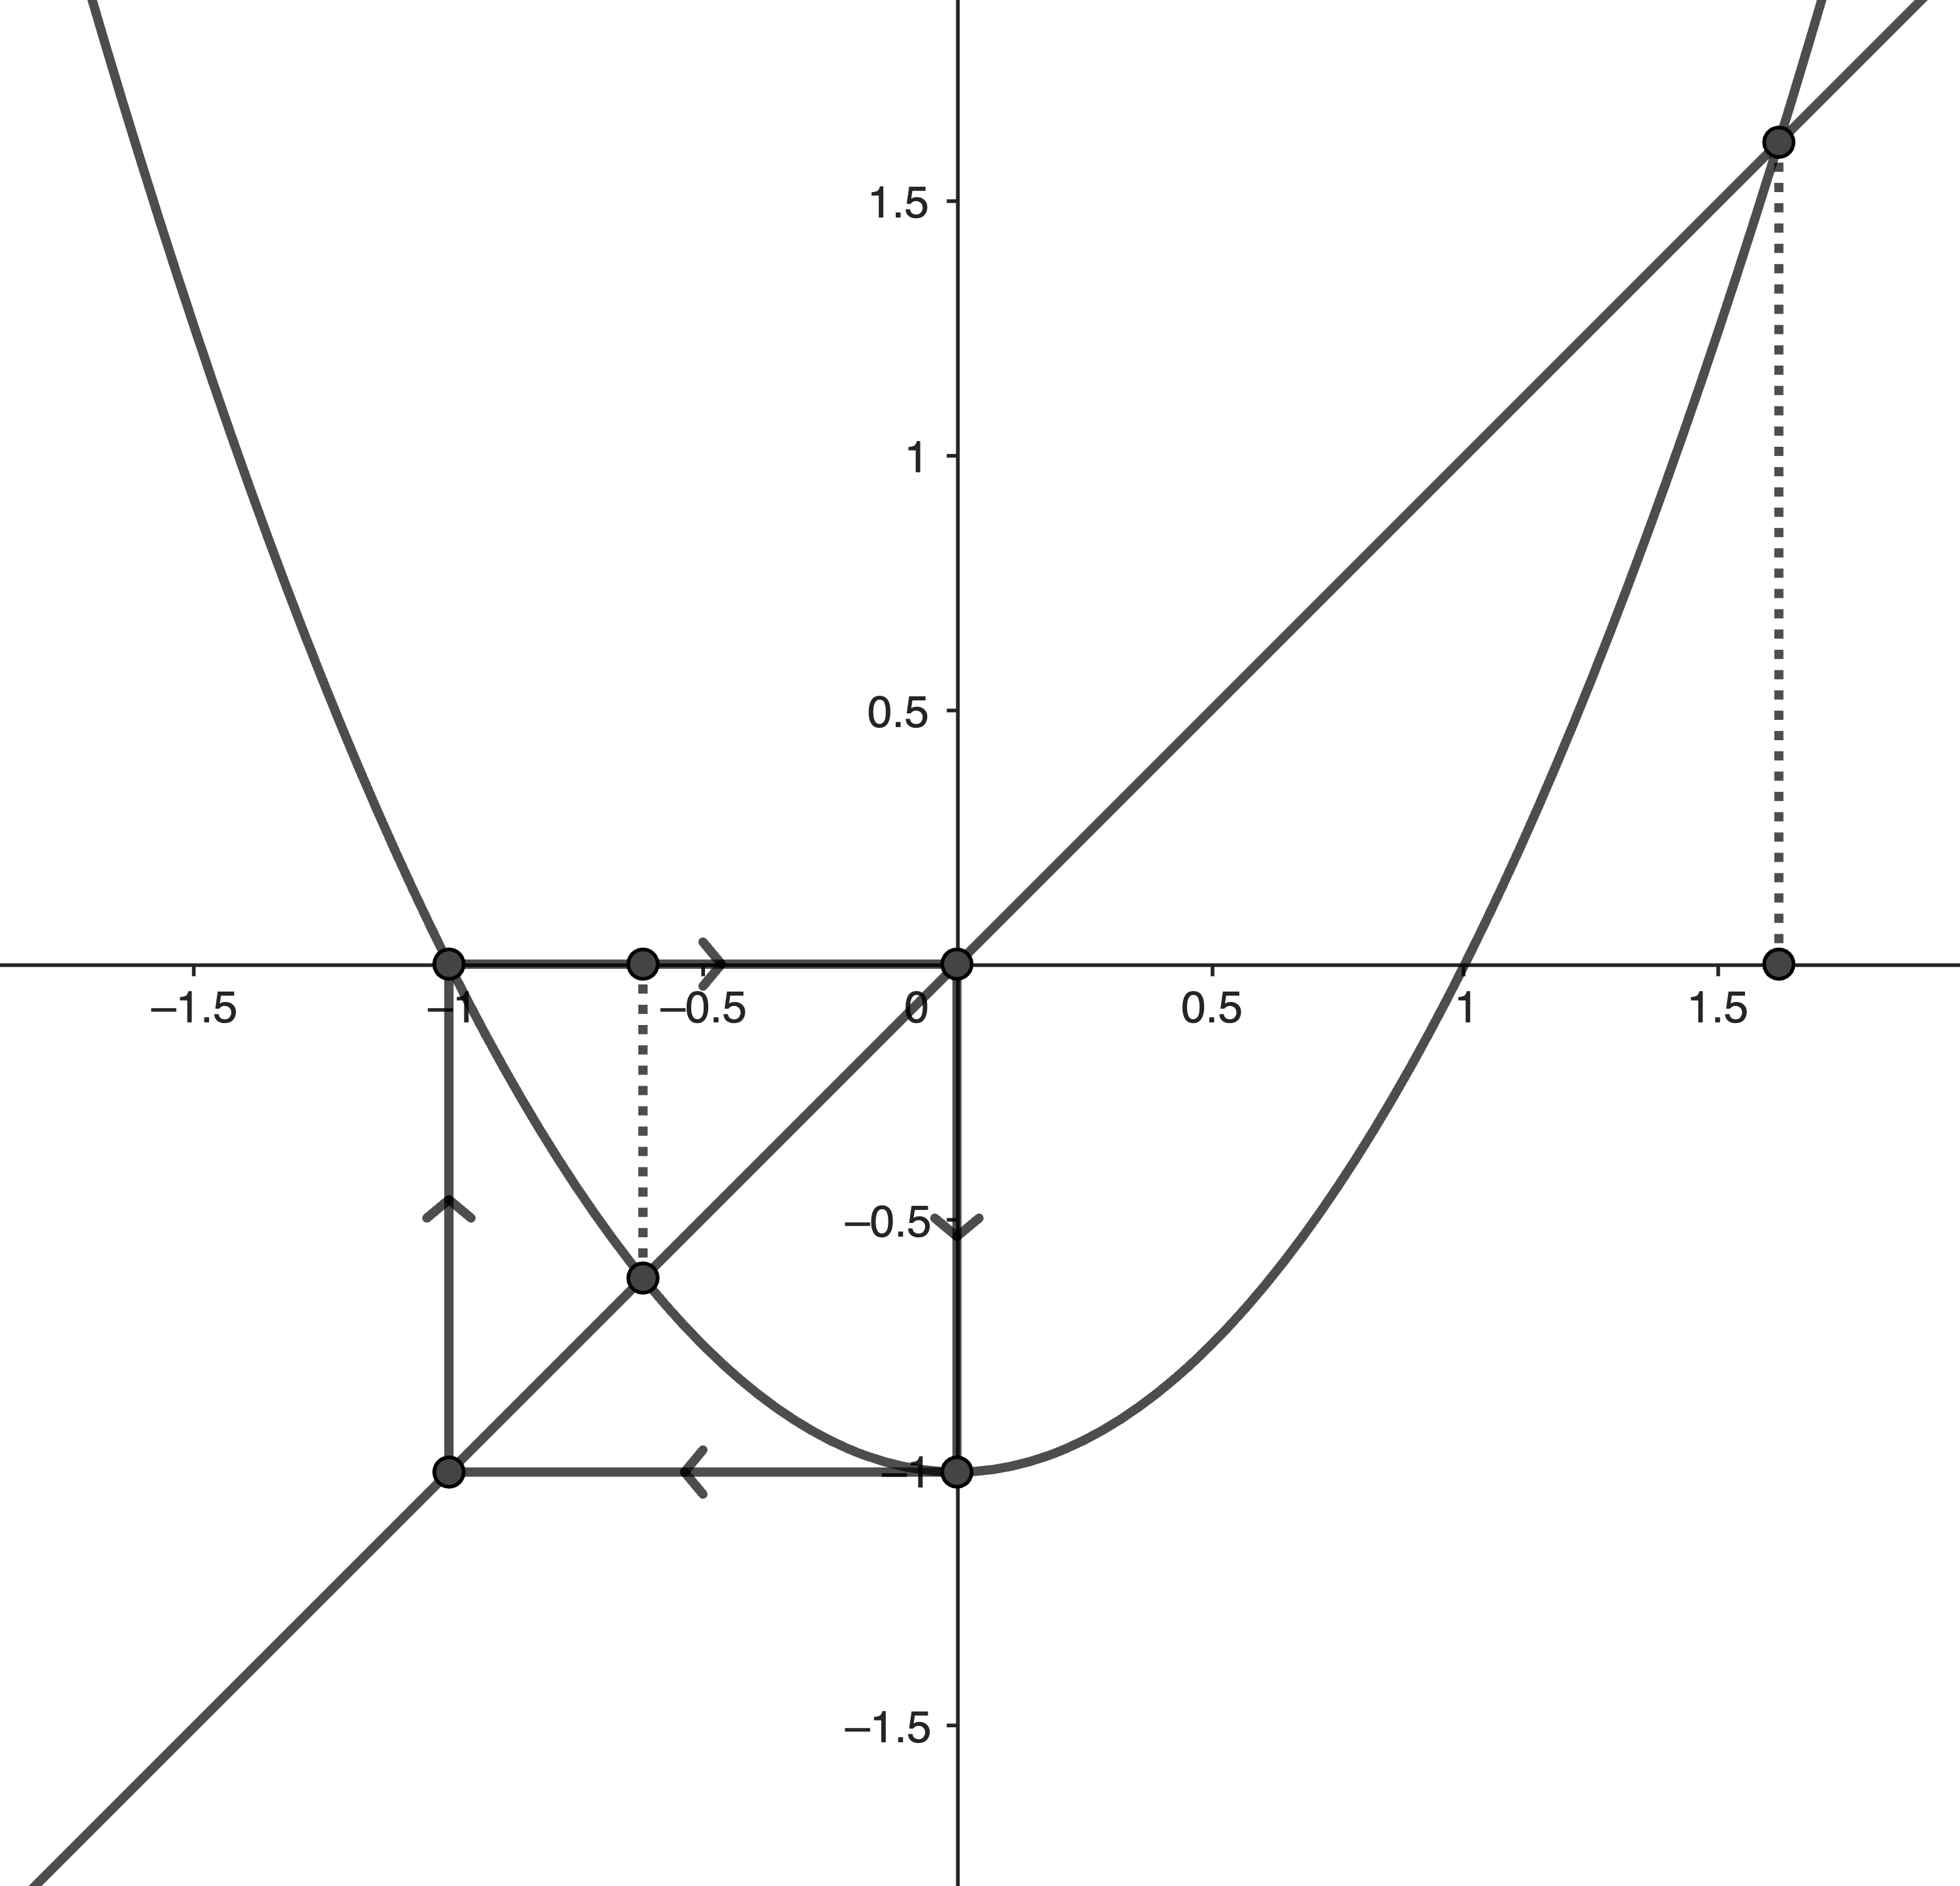
\includegraphics[width=7cm]{ris1}
    \centering
\end{figure}















\section{Асимптотическое поведение}
\textbf{Важно}, что орбита \(x = 0.5\) (любая непериодическая орбита) стремится асимптотически к периодическим орбитам, но за конечное число итераций в нее не приходит.
А на численном счете сказываются ошибки округления.
\\[2mm]
Очень важный результат для конкретной динамической системы это строгое доказательство этого утверждения. 

\section{Периодические орбиты любых периодов}
Отметим, что дискретная динамическая система может обладать периодическими орбитами любого периода.
Например, отображение \(\overline{x} = -\frac{3}{2}x^2 + \frac{5}{2}x + 1\) обладает периодическими орбитами всех периодов.
\\[2mm]
Один из \textbf{центральных вопросов} теории динамических систем --- какова мощность множества периодических точек?

\clm{А.Н. Шарковский, 1964}{
    Если непрерывное отображение интервала имеет периодические орбиты периода 3, то оно имеет периодические орбиты всех периодов больше 3
}{}
